\chapter{Il calore}

Nel capitolo precedente abbiamo definito la \textbf{temperatura} come indice dello stato di agitazione termica di una sostanza. Resta da capire che cosa passa da un corpo caldo a un corpo freddo quando li mettiamo a contatto e le loro temperature si avvicinano. Questo ``qualcosa'' è il \textbf{calore}, e in questo capitolo studiamo che cos'è, come si misura, come si comporta durante i cambiamenti di stato e in quali modi si propaga.

\section[L'energia termica e il calore]{L'energia termica e il calore}

In una fredda giornata d'inverno appoggiamo le mani su un termosifone per scaldarle: qualcosa passa dal termosifone caldo alle nostre mani fredde e ne fa aumentare la temperatura. Se invece stringiamo in mano un cubetto di ghiaccio, è la nostra mano a cedere qualcosa al ghiaccio, e la mano si raffredda.

Abbiamo visto che la temperatura di un corpo è legata alla velocità media delle sue particelle, cioè alla loro \textbf{energia cinetica} microscopica. La somma di tutte queste piccole energie di agitazione disordinata si chiama \textbf{energia termica} (o energia interna) del corpo.

\begin{definizione}
Il \textbf{calore} è l'energia termica che passa spontaneamente da un corpo a temperatura maggiore a un corpo a temperatura minore, per il solo fatto che le loro temperature sono diverse.
\end{definizione}

Conviene tenere ben distinti i due termini: un corpo \emph{possiede} energia termica, due corpi a contatto si \emph{scambiano} calore. Il calore, come il lavoro, è energia \textbf{in transito}: ha senso parlarne solo mentre passa da un corpo all'altro.

\begin{remark}
Essendo una forma di energia, il calore nel Sistema Internazionale si misura in \textbf{joule} (\si{\joule}). In ambito alimentare e medico sopravvive una vecchia unità, la \textbf{caloria} (cal) e il suo multiplo la \textbf{kilocaloria} (kcal, la ``Caloria'' con la C maiuscola delle etichette): $\SI{1}{cal} \approx \SI{4,186}{\joule}$. Una kilocaloria è, con buona approssimazione, il calore che serve per aumentare di \SI{1}{\celsius} la temperatura di un chilogrammo d'acqua.
\end{remark}

\begin{figure}[!htbp]
    \centering
    \begin{tikzpicture}[>=stealth]
        % --- pannello 1: contatto, T diverse ---
        \begin{scope}
            \draw[fill=blue!12] (0,0) rectangle (1.6,1.6);
            \draw[fill=ocre!35] (1.6,0) rectangle (3.4,1.8);
            \node at (0.8,0.8) {\footnotesize $T_1$};
            \node at (2.5,0.9) {\footnotesize $T_2$};
            \node[below,align=center,font=\scriptsize] at (0.8,-0.1) {corpo\\freddo};
            \node[below,align=center,font=\scriptsize] at (2.5,-0.1) {corpo\\caldo};
            \draw[->,very thick,ocre] (2.1,2.15) to[bend right=20] node[midway,above,font=\footnotesize]{$Q$} (1.1,2.15);
            \node[font=\footnotesize] at (1.7,-1.05) {$T_1 < T_2$};
        \end{scope}
        % --- pannello 2: equilibrio ---
        \begin{scope}[xshift=6cm]
            \draw[fill=ocre!18] (0,0) rectangle (1.6,1.6);
            \draw[fill=ocre!18] (1.6,0) rectangle (3.4,1.8);
            \node at (0.8,0.8) {\footnotesize $T_\text{eq}$};
            \node at (2.5,0.9) {\footnotesize $T_\text{eq}$};
            \node[font=\footnotesize] at (1.7,-1.05) {equilibrio termico};
        \end{scope}
    \end{tikzpicture}
    \caption{Due corpi a temperatura diversa messi a contatto: il calore $Q$ passa dal più caldo al più freddo finché le due temperature diventano uguali (equilibrio termico).}
    \label{fig:calore-transito}
\end{figure}

\section[Capacità termica e calore specifico]{Capacità termica e calore specifico}

Se forniamo una certa quantità di calore $Q$ a un corpo, senza che questo cambi stato di aggregazione, la sua temperatura aumenta di una quantità $\Delta T$. L'esperienza mostra che corpi diversi, ricevendo lo stesso calore, si scaldano in modo diverso.

\subsection{La capacità termica}

\begin{definizione}
Il rapporto fra il calore $Q$ fornito a un corpo e l'aumento di temperatura $\Delta T$ che ne consegue si chiama \textbf{capacità termica} $C$ del corpo:
\[ \colorboxed{ocre}{ C = \frac{Q}{\Delta T}. } \]
Si misura in \si{\joule\per\kelvin} (o, indifferentemente, in \si{\joule\per\celsius}).
\end{definizione}

La capacità termica dice quanto calore serve per aumentare di un grado la temperatura di \emph{quel} corpo. Un corpo con grande capacità termica può ricevere molto calore variando di poco la propria temperatura: è il caso di una grande massa d'acqua, come quella di un lago o del mare.

\subsection{Il calore specifico}

Sperimentalmente si verifica che la capacità termica è direttamente proporzionale alla massa: raddoppiando la massa da scaldare, raddoppia il calore necessario per lo stesso $\Delta T$. Il rapporto $C/m$ non dipende quindi dalla quantità di sostanza, ma solo dal materiale.

\begin{definizione}
La \textbf{capacità termica per unità di massa} si chiama \textbf{calore specifico} $c$ della sostanza:
\[ \colorboxed{ocre}{ c = \frac{C}{m}. } \]
Nel Sistema Internazionale si misura in \si{\joule\per\kilogram\per\kelvin}. Rappresenta il calore che serve per aumentare di \SI{1}{\kelvin} la temperatura di \SI{1}{\kilogram} di quella sostanza.
\end{definizione}

\begin{table}[!htbp]
    \centering
    \begin{tabular}{lc}
        \toprule
        sostanza & $c$ $(\si{\joule\per\kilogram\per\kelvin})$ \\
        \midrule
        acqua & $4180$ \\
        alcol etilico & $2430$ \\
        olio d'oliva & $1650$ \\
        aria (a pressione costante) & $\approx 1000$ \\
        alluminio & $880$ \\
        acciaio / ferro & $480$ \\
        rame & $390$ \\
        ottone & $376$ \\
        argento & $238$ \\
        mercurio & $138$ \\
        oro & $134$ \\
        piombo & $128$ \\
        \bottomrule
    \end{tabular}
    \caption{Calore specifico di alcune sostanze, a temperatura ambiente e pressione atmosferica. L'acqua ha un calore specifico eccezionalmente alto.}
    \label{tab:calore-specifico}
\end{table}

\subsection{La legge fondamentale della termologia}

Mettendo insieme le due definizioni ($Q = C\,\Delta T$ e $C = c\,m$) si ottiene la relazione che lega il calore scambiato alla variazione di temperatura:
\[ \colorboxed{ocre}{ Q = c\,m\,\Delta T. } \]

È la \textbf{legge fondamentale della termologia}. Il calore scambiato da un corpo che non cambia stato è:
\begin{itemize}
    \item direttamente proporzionale alla massa $m$;
    \item direttamente proporzionale alla variazione di temperatura $\Delta T$;
    \item legato alla natura della sostanza attraverso il calore specifico $c$.
\end{itemize}
Il segno di $Q$ segue quello di $\Delta T$: se il corpo si scalda ($\Delta T > 0$) assorbe calore ($Q > 0$); se si raffredda ($\Delta T < 0$) cede calore ($Q < 0$).

\begin{remark}
Poiché nelle formule della termologia compaiono sempre \emph{differenze} di temperatura, ed esse valgono lo stesso numero nelle due scale, il calore specifico si può indifferentemente esprimere in \si{\joule\per\kilogram\per\kelvin} o in $\si{\joule\per\kilogram\per\celsius}$, e nei calcoli si può usare $\Delta T$ in kelvin o in gradi Celsius senza cambiare il risultato.
\end{remark}

\begin{testexample}[\thetcbcounter \, L'acqua per la pasta]
Quanto calore serve per portare \SI{2,0}{\kilogram} d'acqua da \SI{18}{\celsius} fino a \SI{100}{\celsius}?

La variazione di temperatura è $\Delta T = 100 - 18 = \SI{82}{\celsius}$. Dalla legge fondamentale:
\[ Q = c\,m\,\Delta T = 4180 \cdot 2{,}0 \cdot 82 \approx \SI{6,9e5}{\joule}. \]
Circa \SI{690}{\kilo\joule}: un fornello da \SI{2}{\kilo\watt} impiega poco più di cinque minuti a fornirli (senza contare le dispersioni).
\end{testexample}

\begin{testexample}[\thetcbcounter \, La capacità termica di una pentola]
Una pentola di acciaio ha massa \SI{0,80}{\kilogram}. Qual è la sua capacità termica? Quanto calore serve per portarla da \SI{20}{\celsius} a \SI{100}{\celsius}?

Il calore specifico dell'acciaio è $c = \SI{480}{\joule\per\kilogram\per\kelvin}$ (tabella~\ref{tab:calore-specifico}), quindi
\[ C = c\,m = 480 \cdot 0{,}80 = \SI{384}{\joule\per\kelvin}. \]
Per un aumento $\Delta T = \SI{80}{\celsius}$ serve
\[ Q = C\,\Delta T = 384 \cdot 80 \approx \SI{3,1e4}{\joule}. \]
Molto meno del calore che assorbe l'acqua contenuta nella pentola: per questo, in prima approssimazione, la capacità termica del recipiente si può spesso trascurare.
\end{testexample}

\begin{testexample}[\thetcbcounter \, Che sostanza è?]
Un blocco metallico di massa \SI{0,50}{\kilogram} assorbe \SI{39,6}{\kilo\joule} e la sua temperatura passa da \SI{20}{\celsius} a \SI{110}{\celsius}. Di che sostanza si tratta?

Ricaviamo il calore specifico dalla legge fondamentale:
\[ c = \frac{Q}{m\,\Delta T} = \frac{\SI{39600}{\joule}}{0{,}50 \cdot 90} = \SI{880}{\joule\per\kilogram\per\kelvin}. \]
Confrontando con la tabella~\ref{tab:calore-specifico}, il blocco è di \textbf{alluminio}.
\end{testexample}

\begin{esercizio}
Quanta energia serve per scaldare \SI{250}{\gram} d'acqua (una tazza) da \SI{20}{\celsius} a \SI{95}{\celsius}?\\
\risp{$Q = 4180 \cdot 0{,}250 \cdot 75 \approx \SI{7,8e4}{\joule}$}
\end{esercizio}

\begin{esercizio}
La piastra di alluminio di un ferro da stiro ha massa \SI{0,60}{\kilogram}. Quanto calore serve per portarla da \SI{20}{\celsius} alla temperatura di lavoro di \SI{180}{\celsius}? ($c_{\text{Al}} = \SI{880}{\joule\per\kilogram\per\kelvin}$)\\
\risp{$Q = 880 \cdot 0{,}60 \cdot 160 \approx \SI{8,4e4}{\joule}$}
\end{esercizio}

\begin{esercizio}
Un blocco di rame di \SI{1,5}{\kilogram} cede \SI{17}{\kilo\joule} raffreddandosi. Di quanti gradi scende la sua temperatura? ($c_{\text{Cu}} = \SI{390}{\joule\per\kilogram\per\kelvin}$)\\
\risp{$\Delta T = \dfrac{Q}{c\,m} = \dfrac{\SI{17000}{\joule}}{390 \cdot 1{,}5} \approx \SI{29}{\celsius}$}
\end{esercizio}

\begin{esercizio}
Un campione di \SI{200}{\gram} di un metallo passa da \SI{25}{\celsius} a \SI{75}{\celsius} assorbendo \SI{1,34}{\kilo\joule}. Calcola il calore specifico e riconosci il metallo dalla tabella~\ref{tab:calore-specifico}.\\
\risp{$c = \dfrac{1340}{0{,}200 \cdot 50} = \SI{134}{\joule\per\kilogram\per\kelvin}$: si tratta di oro}
\end{esercizio}

\begin{esercizio}
Una borsa dell'acqua calda contiene \SI{1,2}{\litre} d'acqua a \SI{70}{\celsius}. Quanto calore cede complessivamente mentre si raffredda fino alla temperatura del corpo, \SI{37}{\celsius}?\\
\risp{$Q = 4180 \cdot 1{,}2 \cdot 33 \approx \SI{1,7e5}{\joule}$ (ceduto)}
\end{esercizio}

\begin{esercizio}
Sullo stesso fornello, che eroga calore a ritmo costante, si scaldano \SI{0,50}{\kilogram} d'acqua e \SI{0,50}{\kilogram} d'olio d'oliva. Quale dei due si scalda prima, e di quante volte più in fretta? ($c_{\text{olio}} = \SI{1650}{\joule\per\kilogram\per\kelvin}$)\\
\risp{l'olio; il rapporto dei calori specifici è $4180/1650 \approx 2{,}5$, quindi l'olio si scalda circa \num{2,5} volte più velocemente}
\end{esercizio}

\section[L'equilibrio termico]{L'equilibrio termico}

Quando due corpi a temperatura diversa sono posti a contatto e isolati dall'ambiente, il calore passa dal più caldo al più freddo finché i due raggiungono la stessa \textbf{temperatura di equilibrio} $T_\text{eq}$, compresa fra le due temperature iniziali.

\subsection{L'equazione dell'equilibrio termico}

Prendiamo una sostanza fredda (massa $m_1$, calore specifico $c_1$, temperatura iniziale $T_1$) e una calda (massa $m_2$, calore specifico $c_2$, temperatura iniziale $T_2 > T_1$). All'equilibrio:
\begin{itemize}
    \item la sostanza fredda si scalda e \emph{acquista} calore: $Q_\text{acq} = c_1\,m_1\,(T_\text{eq} - T_1) > 0$;
    \item la sostanza calda si raffredda e \emph{cede} calore: $Q_\text{ced} = c_2\,m_2\,(T_\text{eq} - T_2) < 0$.
\end{itemize}
Se non ci sono dispersioni verso l'ambiente, tutto il calore ceduto dalla sostanza calda è assorbito da quella fredda. Poiché $Q_\text{ced}$ è negativo e $Q_\text{acq}$ positivo, per uguagliarli bisogna cambiare segno a uno dei due:
\[ \colorboxed{ocre}{ Q_\text{acq} = -\,Q_\text{ced}, \qquad c_1\,m_1\,(T_\text{eq} - T_1) = -\,c_2\,m_2\,(T_\text{eq} - T_2). } \]

Risolvendo rispetto all'incognita $T_\text{eq}$ si ottiene
\[ T_\text{eq} = \frac{c_1\,m_1\,T_1 + c_2\,m_2\,T_2}{c_1\,m_1 + c_2\,m_2}. \]
La temperatura di equilibrio è la \textbf{media dei valori iniziali, pesata con le capacità termiche} $c\,m$ dei due corpi. Se le due sostanze sono uguali ($c_1 = c_2$) l'espressione si semplifica:
\[ T_\text{eq} = \frac{m_1\,T_1 + m_2\,T_2}{m_1 + m_2}. \]

\begin{testexample}[\thetcbcounter \, Due masse d'acqua]
Si mescolano \SI{1,0}{\kilogram} d'acqua a \SI{20}{\celsius} con \SI{3,0}{\kilogram} d'acqua a \SI{60}{\celsius}. Qual è la temperatura finale?

Le sostanze sono identiche, quindi
\[ T_\text{eq} = \frac{m_1\,T_1 + m_2\,T_2}{m_1 + m_2} = \frac{1{,}0 \cdot 20 + 3{,}0 \cdot 60}{1{,}0 + 3{,}0} = \frac{200}{4{,}0} = \SI{50}{\celsius}. \]
La temperatura finale è più vicina a quella della massa maggiore.
\end{testexample}

\begin{testexample}[\thetcbcounter \, Un blocco di ferro nell'acqua]
Un blocco di ferro di massa \SI{0,350}{\kilogram} a \SI{70}{\celsius} viene immerso in \SI{2,0}{\kilogram} d'acqua a \SI{25}{\celsius}. Trascurando le dispersioni e la capacità termica del recipiente, qual è la temperatura di equilibrio? ($c_{\text{Fe}} = 480$, $c_{\text{acqua}} = \SI{4180}{\joule\per\kilogram\per\kelvin}$)

Applichiamo la media pesata con le capacità termiche:
\[ T_\text{eq} = \frac{c_{\text{Fe}}\,m_{\text{Fe}}\,T_{\text{Fe}} + c_{\text{a}}\,m_{\text{a}}\,T_{\text{a}}}{c_{\text{Fe}}\,m_{\text{Fe}} + c_{\text{a}}\,m_{\text{a}}} = \frac{168 \cdot 70 + 8360 \cdot 25}{168 + 8360} \approx \SI{25,9}{\celsius}. \]
La temperatura dell'acqua sale appena, perché la sua capacità termica ($\SI{8360}{\joule\per\kelvin}$) è cinquanta volte quella del blocco di ferro ($\SI{168}{\joule\per\kelvin}$).
\end{testexample}

\subsection{Il calorimetro delle mescolanze}

Non esiste uno strumento che misuri direttamente il calore: lo si ricava da misure di massa e di temperatura. Lo strumento adatto è il \textbf{calorimetro delle mescolanze}, un recipiente a pareti isolanti, con coperchio, provvisto di termometro e di un agitatore per uniformare la temperatura del liquido (figura~\ref{fig:calorimetro}).

\begin{figure}[!htbp]
    \centering
    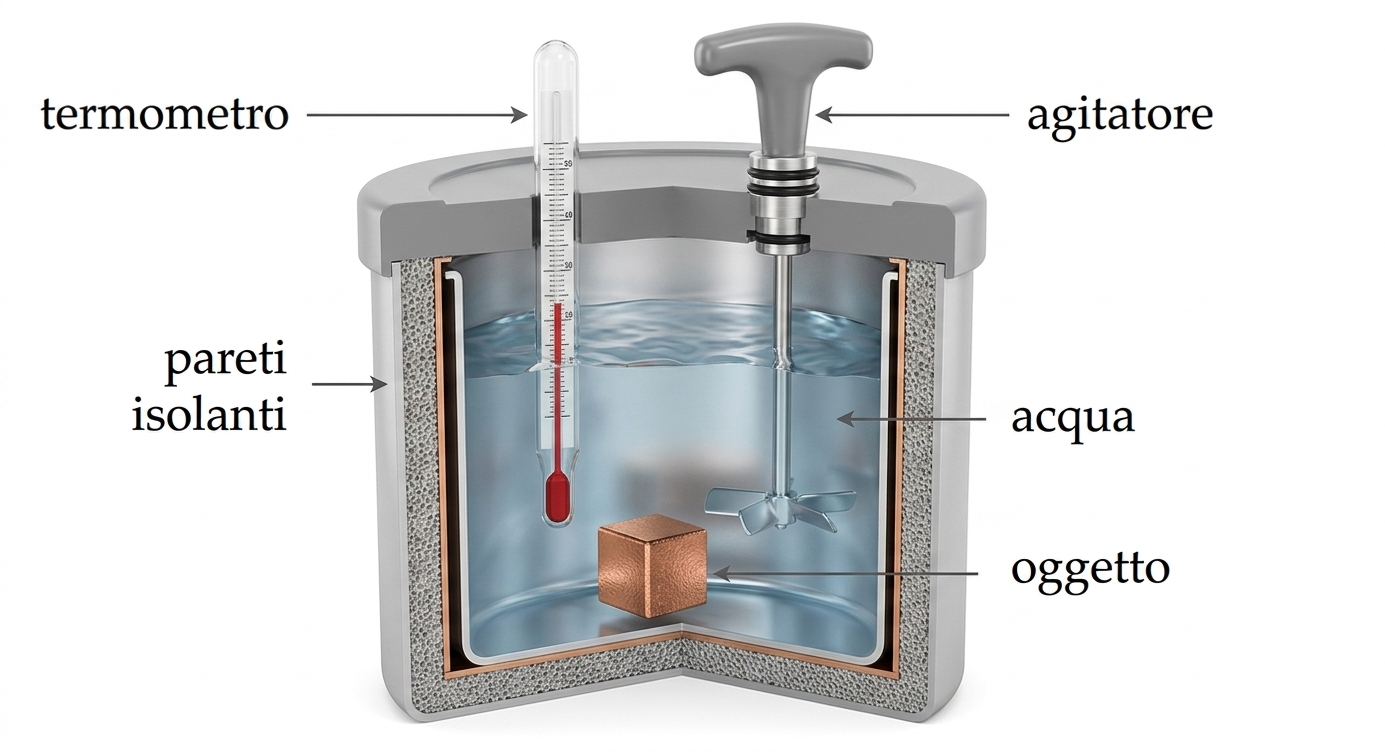
\includegraphics[width=0.78\linewidth]{img/calorimetro.jpg}
    \caption{Il calorimetro delle mescolanze, in sezione: un recipiente a pareti isolanti con coperchio, termometro e agitatore. Immergendo nell'acqua un oggetto caldo e misurando la temperatura di equilibrio si ricava il calore specifico dell'oggetto.}
    \label{fig:calorimetro}
\end{figure}

\textbf{Come si misura il calore specifico di un metallo.} Si versa nel calorimetro una massa nota d'acqua $m_\text{a}$ e se ne misura la temperatura $T_\text{a}$. Si scalda l'oggetto metallico (massa $m_\text{o}$) immergendolo per qualche minuto in acqua bollente, portandolo così a $T_\text{o} = \SI{100}{\celsius}$, e lo si trasferisce rapidamente nel calorimetro. Si agita e si legge la temperatura di equilibrio $T_\text{eq}$. Trascurando la capacità termica del calorimetro, il calore ceduto dall'oggetto è uguale (a parte il segno) a quello assorbito dall'acqua:
\[ c_\text{o}\,m_\text{o}\,(T_\text{eq} - T_\text{o}) = -\,c_\text{a}\,m_\text{a}\,(T_\text{eq} - T_\text{a}), \]
da cui si ricava l'unica incognita $c_\text{o}$.

\begin{testexample}[\thetcbcounter \, Misura al calorimetro]
Nel calorimetro ci sono $m_\text{a} = \SI{0,150}{\kilogram}$ d'acqua a $T_\text{a} = \SI{20}{\celsius}$. Vi si immerge un oggetto di $m_\text{o} = \SI{0,090}{\kilogram}$ portato a $T_\text{o} = \SI{100}{\celsius}$. La temperatura di equilibrio è $T_\text{eq} = \SI{29}{\celsius}$. Qual è il calore specifico dell'oggetto?

Il calore assorbito dall'acqua è
\[ Q_\text{acq} = c_\text{a}\,m_\text{a}\,(T_\text{eq} - T_\text{a}) = 4180 \cdot 0{,}150 \cdot 9 \approx \SI{5643}{\joule}. \]
Questo stesso calore è stato ceduto dall'oggetto, che si è raffreddato da \SI{100}{\celsius} a \SI{29}{\celsius}:
\[ c_\text{o} = \frac{Q_\text{acq}}{m_\text{o}\,(T_\text{o} - T_\text{eq})} = \frac{5643}{0{,}090 \cdot 71} \approx \SI{8,8e2}{\joule\per\kilogram\per\kelvin}. \]
La capacità termica dell'oggetto è $C_\text{o} = c_\text{o}\,m_\text{o} \approx \SI{79}{\joule\per\kelvin}$. Il valore trovato è vicino a quello dell'alluminio.
\end{testexample}

\begin{esercizio}
Si mescolano \SI{2,0}{\kilogram} d'acqua a \SI{80}{\celsius} con \SI{3,0}{\kilogram} d'acqua a \SI{20}{\celsius}. Qual è la temperatura di equilibrio?\\
\risp{$T_\text{eq} = \dfrac{2{,}0 \cdot 80 + 3{,}0 \cdot 20}{5{,}0} = \SI{44}{\celsius}$}
\end{esercizio}

\begin{esercizio}
Per preparare un bagno si riempie la vasca con \SI{40}{\litre} d'acqua a \SI{60}{\celsius} e \SI{20}{\litre} a \SI{18}{\celsius}. Trascurando le dispersioni, qual è la temperatura ottenuta?\\
\risp{$T_\text{eq} = \dfrac{40 \cdot 60 + 20 \cdot 18}{60} = \SI{46}{\celsius}$}
\end{esercizio}

\begin{esercizio}
In una pentola di alluminio di \SI{0,50}{\kilogram} a \SI{20}{\celsius} si versa \SI{1,0}{\kilogram} d'acqua a \SI{90}{\celsius}. Trascurando le dispersioni, a quale temperatura si porta il sistema? ($c_{\text{Al}} = 880$, $c_{\text{acqua}} = \SI{4180}{\joule\per\kilogram\per\kelvin}$)\\
\risp{$T_\text{eq} = \dfrac{440 \cdot 20 + 4180 \cdot 90}{440 + 4180} \approx \SI{83}{\celsius}$}
\end{esercizio}

\begin{esercizio}
A un caffè di \SI{200}{\gram} a \SI{85}{\celsius} si aggiungono \SI{50}{\gram} di latte freddo a \SI{10}{\celsius}. Assumendo per entrambi il calore specifico dell'acqua, qual è la temperatura finale?\\
\risp{$T_\text{eq} = \dfrac{200 \cdot 85 + 50 \cdot 10}{250} = \SI{70}{\celsius}$}
\end{esercizio}

\begin{esercizio}
Un pezzo di rame di \SI{500}{\gram} a \SI{200}{\celsius} viene immerso in \SI{2,0}{\kilogram} d'acqua a \SI{15}{\celsius}. Qual è la temperatura di equilibrio? ($c_{\text{Cu}} = 390$, $c_{\text{acqua}} = \SI{4180}{\joule\per\kilogram\per\kelvin}$)\\
\risp{$T_\text{eq} = \dfrac{195 \cdot 200 + 8360 \cdot 15}{195 + 8360} \approx \SI{19}{\celsius}$}
\end{esercizio}

\begin{esercizio}
Si mescola \SI{1,0}{\kilogram} d'acqua a \SI{15}{\celsius} con una massa d'acqua a \SI{65}{\celsius} e si ottiene una temperatura di equilibrio di \SI{40}{\celsius}. Quanta acqua calda è stata aggiunta?\\
\risp{$m_\text{c}\,(65 - 40) = 1{,}0 \cdot (40 - 15) \Rightarrow m_\text{c} = \SI{1,0}{\kilogram}$}
\end{esercizio}

\begin{esercizio}
Un calorimetro contiene \SI{200}{\gram} d'acqua a \SI{18}{\celsius}. Vi si immerge un blocco di \SI{300}{\gram} di alluminio a \SI{90}{\celsius}. Trascurando la capacità termica del calorimetro, qual è la temperatura di equilibrio? ($c_{\text{Al}} = 880$, $c_{\text{acqua}} = \SI{4180}{\joule\per\kilogram\per\kelvin}$)\\
\risp{$T_\text{eq} = \dfrac{836 \cdot 18 + 264 \cdot 90}{836 + 264} \approx \SI{35}{\celsius}$}
\end{esercizio}

\section[I cambiamenti di stato]{I cambiamenti di stato}

La materia si presenta in tre \textbf{stati di aggregazione}: solido, liquido, aeriforme. Il passaggio da uno stato all'altro si chiama \textbf{cambiamento di stato} (o passaggio di stato) e avviene sempre mediante scambio di calore. I passaggi possibili sono sei, a coppie inverse (figura~\ref{fig:cambiamenti-stato}):
\begin{itemize}
    \item \textbf{fusione} (solido $\to$ liquido) e \textbf{solidificazione} (liquido $\to$ solido);
    \item \textbf{vaporizzazione} (liquido $\to$ aeriforme) e \textbf{condensazione} (aeriforme $\to$ liquido);
    \item \textbf{sublimazione} (solido $\to$ aeriforme) e \textbf{brinamento} (aeriforme $\to$ solido).
\end{itemize}

\begin{figure}[!htbp]
    \centering
    \begin{tikzpicture}[>=stealth,node distance=3.2cm]
        \node[draw,thick,rounded corners,fill=blue!12,minimum width=1.9cm,minimum height=0.9cm] (s) at (0,0) {solido};
        \node[draw,thick,rounded corners,fill=ocre!15,minimum width=1.9cm,minimum height=0.9cm] (l) at (4,0) {liquido};
        \node[draw,thick,rounded corners,fill=red!12,minimum width=1.9cm,minimum height=0.9cm] (g) at (8,0) {aeriforme};
        % fusione / solidificazione
        \draw[->,thick] (s.30) to[bend left=18] node[above,font=\scriptsize]{fusione} (l.150);
        \draw[->,thick] (l.210) to[bend left=18] node[below,font=\scriptsize]{solidificazione} (s.-30);
        % vaporizzazione / condensazione
        \draw[->,thick] (l.30) to[bend left=18] node[above,font=\scriptsize]{vaporizzazione} (g.150);
        \draw[->,thick] (g.210) to[bend left=18] node[below,font=\scriptsize]{condensazione} (l.-30);
        % sublimazione / brinamento
        \draw[->,thick] (s.65) to[bend left=42] node[above,font=\scriptsize]{sublimazione} (g.115);
        \draw[->,thick] (g.245) to[bend left=42] node[below,font=\scriptsize]{brinamento} (s.295);
    \end{tikzpicture}
    \caption{I sei cambiamenti di stato. I passaggi verso stati più disordinati (fusione, vaporizzazione, sublimazione), da sinistra a destra nello schema, richiedono assorbimento di calore; i passaggi inversi lo restituiscono all'ambiente.}
    \label{fig:cambiamenti-stato}
\end{figure}

\begin{definizione}
Durante un cambiamento di stato la \textbf{temperatura della sostanza non varia}: tutto il calore scambiato serve a modificare i legami fra le particelle, non ad aumentarne l'agitazione termica. La temperatura a cui avviene il passaggio (temperatura di fusione, di ebollizione, \dots) è caratteristica della sostanza e della pressione.
\end{definizione}

\subsection{Il calore latente di fusione}

Riscaldiamo un solido: la sua temperatura sale finché raggiunge la \textbf{temperatura di fusione} $T_f$. Da qui in poi il solido comincia a fondere e la temperatura resta \emph{costante} finché tutta la massa è diventata liquida (figura~\ref{fig:curva-riscaldamento}); solo allora un ulteriore apporto di calore fa risalire la temperatura.

\begin{definizione}
Il calore necessario per fondere completamente una massa $m$ di sostanza che si trova già alla temperatura di fusione è direttamente proporzionale a $m$:
\[ \colorboxed{ocre}{ Q = \lambda_f\,m. } \]
La costante $\lambda_f$ si chiama \textbf{calore latente di fusione} e dipende dalla sostanza; si misura in \si{\joule\per\kilogram}.
\end{definizione}

La \textbf{solidificazione} avviene alla stessa temperatura della fusione e restituisce esattamente lo stesso calore: il \textbf{calore latente di solidificazione} è numericamente uguale a quello di fusione. Per fondere \SI{1}{\kilogram} di ghiaccio a \SI{0}{\celsius} servono \SI{334}{\kilo\joule}; quando \SI{1}{\kilogram} d'acqua a \SI{0}{\celsius} solidifica, cede all'ambiente quegli stessi \SI{334}{\kilo\joule}.

\begin{table}[!htbp]
    \centering
    \begin{tabular}{lcc}
        \toprule
        sostanza & $T_f$ $(\si{\celsius})$ & $\lambda_f$ $(\si{\kilo\joule\per\kilogram})$ \\
        \midrule
        acqua (ghiaccio) & $0$ & $334$ \\
        alcol etilico & $-114$ & $105$ \\
        mercurio & $-39$ & $12$ \\
        piombo & $327$ & $23$ \\
        argento & $961$ & $105$ \\
        \bottomrule
    \end{tabular}
    \caption{Temperatura e calore latente di fusione di alcune sostanze, a pressione atmosferica.}
    \label{tab:latente-fusione}
\end{table}

\begin{figure}[!htbp]
    \centering
    \begin{tikzpicture}[>=stealth]
    \begin{axis}[
        width=0.85\linewidth, height=5.4cm,
        xlabel={calore fornito (i tratti non sono in scala)}, ylabel={temperatura (\si{\celsius})},
        xmin=0, xmax=15.5, ymin=-30, ymax=155,
        xtick=\empty, ytick={-20,0,100,140},
        axis lines=left, tick label style={font=\footnotesize},
        label style={font=\footnotesize}, clip=false,
    ]
    \addplot[ocre,very thick] coordinates {(0,-20) (1,0) (4,0) (8,100) (14,100) (15,140)};
    \draw[gray,dashed] (axis cs:1,0) -- (axis cs:1,-20);
    \draw[gray,dashed] (axis cs:8,100) -- (axis cs:8,0);
    \node[font=\scriptsize,anchor=south] at (axis cs:2.5,2) {fusione};
    \node[font=\scriptsize,anchor=south] at (axis cs:11,102) {ebollizione};
    \node[font=\scriptsize,anchor=west] at (axis cs:0.1,-24) {ghiaccio};
    \node[font=\scriptsize,anchor=west] at (axis cs:4.6,55) {acqua};
    \node[font=\scriptsize,anchor=south] at (axis cs:14.6,128) {vapore};
    \end{axis}
    \end{tikzpicture}
    \caption{Curva di riscaldamento dell'acqua, dal ghiaccio sotto zero al vapore. Sui due tratti orizzontali la sostanza cambia stato e la temperatura resta costante, pur continuando a ricevere calore.}
    \label{fig:curva-riscaldamento}
\end{figure}

\subsection{Il calore latente di vaporizzazione}

Il passaggio dallo stato liquido a quello aeriforme può avvenire in due modi. L'\textbf{evaporazione} interessa solo le particelle della superficie libera, avviene a qualsiasi temperatura ed è tanto più rapida quanto più il liquido è caldo e l'aria secca. L'\textbf{ebollizione} interessa tutto il volume del liquido, avviene a una temperatura ben precisa (la \textbf{temperatura di ebollizione}) e la mantiene costante durante tutto il processo.

\begin{definizione}
Il calore necessario per vaporizzare completamente una massa $m$ di liquido che si trova già alla temperatura di ebollizione è
\[ \colorboxed{ocre}{ Q = \lambda_v\,m, } \]
dove $\lambda_v$ è il \textbf{calore latente di vaporizzazione} della sostanza, misurato in \si{\joule\per\kilogram}.
\end{definizione}

Il passaggio inverso, la \textbf{condensazione}, avviene alla stessa temperatura e restituisce lo stesso calore. È per questo che una scottatura da vapore acqueo a \SI{100}{\celsius} è molto più grave di una da acqua liquida alla stessa temperatura: il vapore, condensando sulla pelle, cede in più il suo calore latente ($\lambda_v \approx \SI{2,25e6}{\joule\per\kilogram}$ per l'acqua).

\begin{table}[!htbp]
    \centering
    \begin{tabular}{lcc}
        \toprule
        sostanza & $T_e$ $(\si{\celsius})$ & $\lambda_v$ $(\si{\kilo\joule\per\kilogram})$ \\
        \midrule
        acqua & $100$ & $2250$ \\
        alcol etilico & $78$ & $854$ \\
        mercurio & $357$ & $272$ \\
        piombo & $1750$ & $871$ \\
        \bottomrule
    \end{tabular}
    \caption{Temperatura di ebollizione e calore latente di vaporizzazione, a pressione atmosferica.}
    \label{tab:latente-vaporizzazione}
\end{table}

\subsection{Processi con più passaggi}

La legge fondamentale $Q = c\,m\,\Delta T$ vale solo finché la sostanza non cambia stato. Se durante il riscaldamento è compreso un passaggio di stato, il calore totale è la \textbf{somma} dei calori dei singoli tratti: quelli in cui la temperatura varia ($c\,m\,\Delta T$, con il calore specifico dello stato giusto) e quelli in cui avviene il cambiamento di stato ($\lambda\,m$, a temperatura costante).

\begin{testexample}[\thetcbcounter \, Fondere il ghiaccio]
Quanto calore serve per fondere completamente \SI{2,0}{\kilogram} di ghiaccio che si trova già a \SI{0}{\celsius}? ($\lambda_f = \SI{334}{\kilo\joule\per\kilogram}$)
\[ Q = \lambda_f\,m = \SI{334e3}{\joule\per\kilogram} \cdot \SI{2,0}{\kilogram} = \SI{6,7e5}{\joule}. \]
\end{testexample}

\begin{testexample}[\thetcbcounter \, Dal ghiaccio all'acqua tiepida]
Vogliamo portare \SI{500}{\gram} di ghiaccio da \SI{-10}{\celsius} fino ad acqua a \SI{20}{\celsius}. Quanto calore serve? ($c_{\text{ghiaccio}} = 2100$, $c_{\text{acqua}} = 4180$, in \si{\joule\per\kilogram\per\kelvin}; $\lambda_f = \SI{334}{\kilo\joule\per\kilogram}$)

Il processo ha tre tratti:
\begin{itemize}
    \item riscaldamento del ghiaccio da \SI{-10}{\celsius} a \SI{0}{\celsius}:
    \[ Q_1 = c_{\text{gh}}\,m\,\Delta T = 2100 \cdot 0{,}500 \cdot 10 = \SI{10500}{\joule}; \]
    \item fusione a \SI{0}{\celsius}:
    \[ Q_2 = \lambda_f\,m = \SI{334e3}{} \cdot 0{,}500 = \SI{167000}{\joule}; \]
    \item riscaldamento dell'acqua da \SI{0}{\celsius} a \SI{20}{\celsius}:
    \[ Q_3 = c_{\text{a}}\,m\,\Delta T = 4180 \cdot 0{,}500 \cdot 20 = \SI{41800}{\joule}. \]
\end{itemize}
In totale $Q = Q_1 + Q_2 + Q_3 \approx \SI{2,2e5}{\joule}$. Si noti che la sola fusione richiede più calore del riscaldamento dell'acqua di venti gradi: sciogliere il ghiaccio ``costa'' molto.
\end{testexample}

\begin{testexample}[\thetcbcounter \, Evaporare l'acqua di una pentola]
Quanto calore serve per far evaporare completamente \SI{200}{\gram} d'acqua che si trova già a \SI{100}{\celsius}? ($\lambda_v = \SI{2250}{\kilo\joule\per\kilogram}$)
\[ Q = \lambda_v\,m = \SI{2,25e6}{} \cdot 0{,}200 \approx \SI{4,5e5}{\joule}. \]
Più del calore che è servito per portare la stessa acqua da temperatura ambiente fino all'ebollizione: l'ultima parte della cottura, quella in cui l'acqua ``se ne va'', è la più dispendiosa.
\end{testexample}

\begin{testexample}[\thetcbcounter \, Il calore prodotto dagli sci]
Quando gli sci scorrono sulla neve, l'attrito produce calore e fonde un sottile velo di neve, che li fa scivolare meglio. Uno sciatore preme sulla neve (a \SI{0}{\celsius}) con una forza normale complessiva $F_n = \SI{800}{\newton}$; il coefficiente di attrito radente è $k_r = 0{,}10$. Quale distanza deve percorrere per fondere \SI{1,0}{\kilogram} di neve? ($\lambda_f = \SI{334}{\kilo\joule\per\kilogram}$)

Il calore prodotto è uguale al lavoro della forza di attrito, $Q = F_n\,k_r\,d$. Il calore che serve per fondere \SI{1,0}{\kilogram} di neve già a \SI{0}{\celsius} è $Q = \lambda_f\,m = \SI{334}{\kilo\joule}$. Uguagliando:
\[ d = \frac{\lambda_f\,m}{F_n\,k_r} = \frac{\SI{334000}{\joule}}{800 \cdot 0{,}10} \approx \SI{4,2e3}{\metre} \approx \SI{4,2}{\kilo\metre}. \]
Serve moltissimo lavoro meccanico per fondere anche solo un chilogrammo di ghiaccio: nella realtà buona parte del calore d'attrito riscalda gli sci e l'aria, e il velo d'acqua si forma solo grazie all'alta pressione locale sotto la lamina.
\end{testexample}

\begin{esercizio}
Quanto calore serve per fondere \SI{500}{\gram} di piombo che si trova già alla temperatura di fusione? ($\lambda_f = \SI{23}{\kilo\joule\per\kilogram}$)\\
\risp{$Q = \SI{23e3}{} \cdot 0{,}500 \approx \SI{1,2e4}{\joule}$}
\end{esercizio}

\begin{esercizio}
Si fa evaporare completamente \SI{1,0}{\kilogram} d'acqua che bolle a \SI{100}{\celsius}. Quanto calore assorbe? ($\lambda_v = \SI{2250}{\kilo\joule\per\kilogram}$)\\
\risp{$Q = \lambda_v\,m = \SI{2,25e6}{\joule}$}
\end{esercizio}

\begin{esercizio}
Un cubetto di ghiaccio di \SI{30}{\gram} a \SI{0}{\celsius} si scioglie del tutto nel bicchiere. Quanto calore ha assorbito dall'ambiente? ($\lambda_f = \SI{334}{\kilo\joule\per\kilogram}$)\\
\risp{$Q = \SI{334e3}{} \cdot 0{,}030 \approx \SI{1,0e4}{\joule}$}
\end{esercizio}

\begin{esercizio}
Quanto calore serve per portare \SI{200}{\gram} di ghiaccio da \SI{-18}{\celsius} (temperatura del congelatore) fino a \SI{0}{\celsius}, senza fonderlo? ($c_{\text{ghiaccio}} = \SI{2100}{\joule\per\kilogram\per\kelvin}$)\\
\risp{$Q = 2100 \cdot 0{,}200 \cdot 18 \approx \SI{7,6e3}{\joule}$}
\end{esercizio}

\begin{esercizio}
Quanto calore serve per trasformare \SI{100}{\gram} di ghiaccio a \SI{0}{\celsius} in acqua a \SI{100}{\celsius}? ($\lambda_f = 334$, in \si{\kilo\joule\per\kilogram}; $c_{\text{acqua}} = \SI{4180}{\joule\per\kilogram\per\kelvin}$)\\
\risp{$Q = \lambda_f\,m + c\,m\,\Delta T = 33400 + 41800 \approx \SI{7,5e4}{\joule}$}
\end{esercizio}

\begin{esercizio}
Un martello di acciaio batte un chiodo di \SI{50}{\gram} ($c = \SI{480}{\joule\per\kilogram\per\kelvin}$); a ogni colpo il \SI{60}{\percent} dell'energia meccanica del colpo (\SI{200}{\joule}) diventa calore nel chiodo. Di quanto sale la temperatura del chiodo dopo \num{20} colpi?\\
\risp{$Q = 0{,}60 \cdot 200 \cdot 20 = \SI{2400}{\joule}$; \; $\Delta T = Q/(c\,m) = 2400/(0{,}050 \cdot 480) = \SI{100}{\celsius}$}
\end{esercizio}

\begin{esercizio}
Una piastra a induzione da \SI{2,0}{\kilo\watt} riceve \SI{1,5}{\kilogram} d'acqua a \SI{20}{\celsius}. Quanto tempo impiega a portarla all'ebollizione e poi a farne evaporare \SI{0,50}{\kilogram}? ($c_{\text{acqua}} = 4180$, $\lambda_v = \SI{2,25e6}{}$, in unità SI)\\
\risp{$Q_1 = 4180 \cdot 1{,}5 \cdot 80 \approx \SI{5,0e5}{\joule}$; \; $Q_2 = \SI{2,25e6}{} \cdot 0{,}50 \approx \SI{1,13e6}{\joule}$; \; $t = (Q_1+Q_2)/P \approx \SI{813}{\second} \approx \SI{14}{\minute}$}
\end{esercizio}

\section[La propagazione del calore]{La propagazione del calore}

Il calore si trasmette da un corpo caldo a uno freddo in tre modi diversi: per \textbf{conduzione}, per \textbf{convezione} e per \textbf{irraggiamento}.

\subsection{La conduzione}

Se scaldiamo con una fiamma l'estremità di una sbarra metallica, dopo un po' anche l'altra estremità diventa calda: il calore si è propagato per \textbf{conduzione}. Gli atomi della zona calda vibrano più intensamente e, urtando i vicini, trasmettono loro l'energia di vibrazione, di atomo in atomo, senza che ci sia trasporto di materia. È il meccanismo tipico dei \textbf{solidi}, in particolare dei metalli.

\begin{definizione}
\textbf{Legge di Fourier.} La quantità di calore $Q$ che attraversa per conduzione una parete piana di spessore $d$ e area $A$, le cui facce sono mantenute a temperature che differiscono di $\Delta T$, nell'intervallo di tempo $\Delta t$ è:
\[ \colorboxed{ocre}{ Q = \frac{k\,A\,\Delta T\,\Delta t}{d}. } \]
Il coefficiente $k$ si chiama \textbf{conducibilità termica} e dipende dal materiale della parete; si misura in \si{\watt\per\metre\per\kelvin}.
\end{definizione}

Il calore che passa è tanto maggiore quanto più grandi sono l'area, la differenza di temperatura e il tempo, e quanto più sottile è la parete. Dividendo per $\Delta t$ si ottiene la \textbf{potenza termica} trasmessa:
\[ P = \frac{Q}{\Delta t} = \frac{k\,A\,\Delta T}{d}. \]

\begin{figure}[!htbp]
    \centering
    \begin{tikzpicture}[>=stealth]
        % parete
        \draw[thick,fill=gray!20] (0,0) rectangle (1.2,3.2);
        \node[font=\footnotesize] at (0.6,-0.35) {$d$};
        \draw[<->] (0,-0.05) -- (1.2,-0.05);
        \node[font=\footnotesize,align=center] at (0.6,1.6) {area\\$A$};
        % faccia calda
        \node[left,ocre!80!black,font=\footnotesize] at (-0.2,3.0) {$T_2$ (calda)};
        % faccia fredda
        \node[right,blue!60!black,font=\footnotesize] at (1.4,0.3) {$T_1$ (fredda)};
        % frecce di calore
        \foreach \y in {0.5,1.1,1.7,2.3,2.9}{
            \draw[->,thick,ocre] (-1.1,\y) -- (-0.05,\y);
            \draw[->,thick,ocre!45] (1.25,\y) -- (2.3,\y);
        }
        \node[font=\footnotesize] at (1.7,3.0) {$Q$};
    \end{tikzpicture}
    \caption{Conduzione attraverso una parete piana. Il calore fluisce dalla faccia calda a quella fredda con una potenza $P = k\,A\,\Delta T / d$: cresce con l'area e con $\Delta T$, diminuisce con lo spessore.}
    \label{fig:conduzione}
\end{figure}

\begin{remark}
Le sostanze che conducono bene il calore ($k$ grande) si dicono \textbf{conduttori termici}: sono i metalli. Quelle che lo conducono male ($k$ piccolo) sono gli \textbf{isolanti termici}: legno, polistirolo, sughero, lana, e soprattutto l'\textbf{aria immobile}. I materiali isolanti da costruzione (mattoni forati, pannelli espansi, doppi vetri) devono la loro efficacia proprio all'aria ferma intrappolata al loro interno. Nei problemi si assume che le due facce della parete siano a temperatura nota: in realtà un sottile strato d'aria aderente a ciascuna faccia riduce ulteriormente il flusso.
\end{remark}

\begin{table}[!htbp]
    \centering
    \begin{tabular}{lc}
        \toprule
        sostanza & $k$ $(\si{\watt\per\metre\per\kelvin})$ \\
        \midrule
        argento & $430$ \\
        rame & $390$ \\
        alluminio & $235$ \\
        ferro & $67$ \\
        vetro & $0{,}6 \div 0{,}9$ \\
        mattone pieno & $\approx 0{,}6$ \\
        acqua & $\approx 0{,}6$ \\
        legno & $0{,}1 \div 0{,}4$ \\
        sughero & $\approx 0{,}045$ \\
        aria (immobile) & $\approx 0{,}026$ \\
        \bottomrule
    \end{tabular}
    \caption{Conducibilità termica di alcune sostanze. Fra i metalli e gli isolanti ci sono quattro ordini di grandezza di differenza.}
    \label{tab:conducibilita}
\end{table}

\begin{testexample}[\thetcbcounter \, Il calore che esce da una parete]
Una parete di mattoni ($k = \SI{0,60}{\watt\per\metre\per\kelvin}$) è spessa \SI{20}{\centi\metre} e ha superficie \SI{12}{\metre\squared}. Dentro la stanza ci sono \SI{20}{\celsius}, fuori \SI{4}{\celsius}. Quanto calore attraversa la parete in un'ora? Quale potenza si disperde?

La differenza di temperatura è $\Delta T = \SI{16}{\celsius}$ e $\Delta t = \SI{3600}{\second}$. Per la legge di Fourier:
\[ Q = \frac{k\,A\,\Delta T\,\Delta t}{d} = \frac{0{,}60 \cdot 12 \cdot 16 \cdot 3600}{0{,}20} \approx \SI{2,1e6}{\joule}. \]
La potenza dispersa è
\[ P = \frac{Q}{\Delta t} = \frac{k\,A\,\Delta T}{d} = \frac{0{,}60 \cdot 12 \cdot 16}{0{,}20} \approx \SI{576}{\watt}. \]
\end{testexample}

\begin{testexample}[\thetcbcounter \, Perché le finestre disperdono tanto]
Una parete di una casa ha superficie totale \SI{60}{\metre\squared} e spessore $d_m = \SI{20}{\centi\metre}$; di questa, \SI{20}{\metre\squared} sono finestre di vetro spesse $d_v = \SI{4,0}{\milli\metre}$. Sapendo che la conducibilità del muro è \num{5} volte quella del vetro, quale frazione del calore si disperde attraverso le finestre?

Il muro ``pieno'' ha area $A_m = 60 - 20 = \SI{40}{\metre\squared}$. A parità di $\Delta T$ e di $\Delta t$, il rapporto fra i calori che passano dal vetro e dal muro è
\[ \frac{Q_v}{Q_m} = \frac{A_v / d_v}{A_m \cdot 5 / d_m} = \frac{20 / 0{,}0040}{40 \cdot 5 / 0{,}20} = \frac{5000}{1000} = 5. \]
Quindi $Q_v = 5\,Q_m$: sul totale $Q_v + Q_m = 6\,Q_m$, le finestre disperdono $5/6 \approx \SI{83}{\percent}$ del calore, pur occupando solo un terzo della superficie. Ecco perché conviene investire nei doppi vetri.
\end{testexample}

\subsection{La convezione}

Se scaldiamo dell'acqua in una pentola, il fondo si scalda per conduzione; l'acqua a contatto con il fondo si dilata, diventa meno densa e sale, mentre l'acqua fredda più in alto scende a prenderne il posto. Si formano così dei moti circolatori, le \textbf{correnti convettive}, che rimescolano il fluido e trasportano il calore in tutto il volume.

\begin{definizione}
La \textbf{convezione} è la propagazione del calore che avviene nei \textbf{fluidi} (liquidi e gas) tramite spostamento di materia: le porzioni calde di fluido, più leggere, salgono; quelle fredde, più pesanti, scendono.
\end{definizione}

La convezione spiega molti fenomeni quotidiani: il termosifone si mette in basso e il condizionatore in alto, perché l'aria calda sale e quella fredda scende; le brezze di mare e di terra; il tiraggio di un camino. Quando il fluido è mosso anche da un agente esterno (un ventilatore, una pompa) si parla di \textbf{convezione forzata}.

\begin{figure}[!htbp]
    \centering
    \begin{tikzpicture}[>=stealth]
        % pentola
        \draw[thick] (0,0) -- (0,2.4) (3.2,0) -- (3.2,2.4);
        \draw[thick] (0,0) -- (3.2,0);
        \fill[blue!12] (0.05,0.05) rectangle (3.15,2.2);
        \draw[blue!35] (0.05,2.2) -- (3.15,2.2);
        % fiamma
        \foreach \x in {1.0,1.6,2.2}{
            \draw[red!70!black,thick] (\x,-0.05) .. controls (\x-0.12,-0.35) and (\x+0.12,-0.5) .. (\x,-0.75);
        }
        % correnti convettive
        \draw[->,thick,ocre] (1.6,0.3) -- (1.6,1.9);
        \draw[->,thick,blue!60!black] (0.5,1.9) .. controls (0.5,0.6) .. (1.3,0.35);
        \draw[->,thick,blue!60!black] (2.7,1.9) .. controls (2.7,0.6) .. (1.9,0.35);
        \draw[->,thick,ocre] (1.6,1.9) .. controls (1.2,2.05) .. (0.7,1.85);
        \draw[->,thick,ocre] (1.6,1.9) .. controls (2.0,2.05) .. (2.5,1.85);
        \node[font=\scriptsize,ocre!80!black] at (2.05,1.25) {caldo};
        \node[font=\scriptsize,blue!60!black] at (0.62,1.35) {freddo};
    \end{tikzpicture}
    \caption{Correnti convettive in una pentola d'acqua sul fuoco: l'acqua calda sale al centro, quella fredda scende lungo le pareti. Il calore si distribuisce così in tutto il liquido.}
    \label{fig:convezione}
\end{figure}

\subsection{L'irraggiamento}

Il calore del Sole ci raggiunge attraverso lo spazio vuoto, dove non c'è materia: né conduzione né convezione sono possibili. Il meccanismo è l'\textbf{irraggiamento}: ogni corpo emette \textbf{onde elettromagnetiche} (per i corpi caldi ma non incandescenti, soprattutto radiazione infrarossa) che trasportano energia e possono propagarsi anche nel vuoto.

\begin{definizione}
La potenza $P$ irraggiata da un corpo è proporzionale all'area $A$ della superficie emittente e alla \textbf{quarta potenza della temperatura assoluta} $T$ (\textbf{legge di Stefan--Boltzmann}):
\[ \colorboxed{ocre}{ P = \frac{Q}{\Delta t} = c\,A\,T^4, } \]
dove la costante $c$ dipende dalla natura della superficie (massima per un corpo nero, minore per una superficie chiara e lucida).
\end{definizione}

La dipendenza da $T^4$ è molto forte: raddoppiando la temperatura assoluta, la potenza irraggiata diventa $2^4 = 16$ volte più grande. Quando la radiazione raggiunge un corpo, in parte viene assorbita (e lo riscalda), in parte riflessa, in parte -- se il corpo è trasparente -- trasmessa. Le superfici scure e opache assorbono bene ed emettono bene; quelle chiare e lucide riflettono e trattengono il calore: è il principio della coperta termica di emergenza (un foglio metallizzato) e del rivestimento a specchio dei thermos.

\begin{figure}[!htbp]
    \centering
    \begin{tikzpicture}[>=stealth]
        % corpo caldo
        \draw[thick,fill=ocre!45] (0,0) circle (0.7);
        \node[font=\scriptsize] at (0,0) {$T$};
        % raggi ondulati in tutte le direzioni
        \foreach \a in {0,45,90,135,180,225,270,315}{
            \draw[ocre,thick,decorate,decoration={snake,amplitude=0.6pt,segment length=4pt}]
                (\a:0.8) -- (\a:2.0);
            \draw[->,ocre] (\a:1.95) -- (\a:2.15);
        }
        \node[font=\footnotesize,anchor=west] at (2.3,-0.9) {onde elettromagnetiche};
    \end{tikzpicture}
    \caption{Irraggiamento: un corpo a temperatura $T$ emette onde elettromagnetiche in tutte le direzioni, con potenza proporzionale a $A\,T^4$. La trasmissione avviene anche in assenza di materia.}
    \label{fig:irraggiamento}
\end{figure}

\begin{testexample}[\thetcbcounter \, Una barra che si scalda]
Una barra metallica irraggia una potenza di \SI{5,0}{\watt} quando la sua superficie è alla temperatura assoluta di \SI{300}{\kelvin}. Quale potenza irraggerebbe a \SI{350}{\kelvin}?

Per la legge di Stefan--Boltzmann la potenza è proporzionale a $T^4$, quindi
\[ \frac{P_2}{P_1} = \left(\frac{T_2}{T_1}\right)^4 = \left(\frac{350}{300}\right)^4 \approx 1{,}85, \qquad P_2 \approx 5{,}0 \cdot 1{,}85 \approx \SI{9,3}{\watt}. \]
Un aumento di temperatura di appena il \SI{17}{\percent} quasi raddoppia la potenza irraggiata.
\end{testexample}

\begin{esercizio}
Una parete di mattoni forati ($k = \SI{0,50}{\watt\per\metre\per\kelvin}$) è spessa \SI{25}{\centi\metre} e ha superficie \SI{15}{\metre\squared}. Le sue facce sono a \SI{19}{\celsius} e a \SI{6}{\celsius}. Quanto calore la attraversa in un'ora?\\
\risp{$Q = \dfrac{0{,}50 \cdot 15 \cdot 13 \cdot 3600}{0{,}25} \approx \SI{1,4e6}{\joule}$}
\end{esercizio}

\begin{esercizio}
Per la stessa parete dell'esercizio precedente, qual è la potenza termica dispersa?\\
\risp{$P = \dfrac{Q}{\Delta t} = \dfrac{0{,}50 \cdot 15 \cdot 13}{0{,}25} \approx \SI{390}{\watt}$}
\end{esercizio}

\begin{esercizio}
Un pannello di sughero ($k = \SI{0,045}{\watt\per\metre\per\kelvin}$) è spesso \SI{5,0}{\centi\metre} e ha superficie \SI{8,0}{\metre\squared}; la differenza di temperatura fra le due facce è \SI{18}{\celsius}. Quale potenza lo attraversa?\\
\risp{$P = \dfrac{0{,}045 \cdot 8{,}0 \cdot 18}{0{,}050} \approx \SI{1,3e2}{\watt}$}
\end{esercizio}

\begin{esercizio}
Perché un pavimento di piastrelle sembra più freddo di un tappeto che si trova alla stessa temperatura?\\
\risp{le piastrelle hanno conducibilità termica molto maggiore: sottraggono calore al piede più in fretta, e la sensazione di freddo dipende dalla \emph{rapidità} con cui il calore lascia la pelle}
\end{esercizio}

\begin{esercizio}
Perché i termosifoni si installano in basso, sotto le finestre, e gli split del condizionatore in alto?\\
\risp{per sfruttare la convezione: l'aria calda del termosifone sale e scalda tutta la stanza; l'aria fredda del condizionatore scende. Mettendoli al contrario, l'aria trattata resterebbe vicino all'apparecchio}
\end{esercizio}

\begin{esercizio}
Una stufa irraggia \SI{800}{\watt} quando la sua superficie è a \SI{400}{\kelvin}. Quale potenza irraggerebbe a \SI{500}{\kelvin}?\\
\risp{$P_2 = 800 \cdot (500/400)^4 \approx \SI{2,0e3}{\watt}$}
\end{esercizio}

\begin{esercizio}
Un thermos ha una doppia parete di vetro con il vuoto nell'intercapedine e le superfici argentate. Come agisce contro ciascuno dei tre meccanismi di propagazione del calore?\\
\risp{il vuoto elimina conduzione e convezione (non c'è materia nell'intercapedine); le superfici argentate, lucide, riflettono la radiazione infrarossa e riducono l'irraggiamento}
\end{esercizio}

\section{Problemi di riepilogo}

\begin{esercizio}
Quanto calore serve per scaldare \SI{300}{\gram} d'acqua da \SI{15}{\celsius} a \SI{100}{\celsius}?\\
\risp{$Q = 4180 \cdot 0{,}300 \cdot 85 \approx \SI{1,1e5}{\joule}$}
\end{esercizio}

\begin{esercizio}
Un blocco di rame di \SI{2,0}{\kilogram} ($c = \SI{390}{\joule\per\kilogram\per\kelvin}$) assorbe \SI{47}{\kilo\joule} partendo da \SI{25}{\celsius}. A quale temperatura arriva?\\
\risp{$\Delta T = 47000/(2{,}0 \cdot 390) \approx \SI{60}{\celsius}$; \; $T \approx \SI{85}{\celsius}$}
\end{esercizio}

\begin{esercizio}
Un campione di \SI{250}{\gram} di metallo passa da \SI{20}{\celsius} a \SI{70}{\celsius} assorbendo \SI{1,60}{\kilo\joule}. Qual è il calore specifico? Di che metallo si tratta?\\
\risp{$c = 1600/(0{,}250 \cdot 50) = \SI{128}{\joule\per\kilogram\per\kelvin}$: piombo}
\end{esercizio}

\begin{esercizio}
Qual è la capacità termica di \SI{1,5}{\litre} d'acqua?\\
\risp{$C = c\,m = 4180 \cdot 1{,}5 \approx \SI{6,3e3}{\joule\per\kelvin}$}
\end{esercizio}

\begin{esercizio}
Si mescolano \SI{1,0}{\kilogram} d'acqua a \SI{90}{\celsius} con \SI{4,0}{\kilogram} a \SI{15}{\celsius}. Qual è la temperatura di equilibrio?\\
\risp{$T_\text{eq} = \dfrac{1{,}0 \cdot 90 + 4{,}0 \cdot 15}{5{,}0} = \SI{30}{\celsius}$}
\end{esercizio}

\begin{esercizio}
Un blocco di ferro di \SI{0,80}{\kilogram} a \SI{250}{\celsius} viene immerso in \SI{3,0}{\litre} d'acqua a \SI{20}{\celsius}. Trascurando le dispersioni, qual è la temperatura di equilibrio? ($c_{\text{Fe}} = 480$, $c_{\text{acqua}} = \SI{4180}{\joule\per\kilogram\per\kelvin}$)\\
\risp{$T_\text{eq} = \dfrac{384 \cdot 250 + 12540 \cdot 20}{384 + 12540} \approx \SI{27}{\celsius}$}
\end{esercizio}

\begin{esercizio}
Un calorimetro contiene \SI{200}{\gram} d'acqua a \SI{20}{\celsius}. Vi si immerge un blocco di \SI{250}{\gram} di ottone a \SI{95}{\celsius}. Trascurando la capacità termica del calorimetro, a quale temperatura si porta il sistema? ($c_{\text{ottone}} = 376$, $c_{\text{acqua}} = \SI{4180}{\joule\per\kilogram\per\kelvin}$)\\
\risp{$T_\text{eq} = \dfrac{836 \cdot 20 + 94 \cdot 95}{836 + 94} \approx \SI{28}{\celsius}$}
\end{esercizio}

\begin{esercizio}
Un asciugacapelli eroga \SI{1,8}{\kilo\watt}. Se il \SI{70}{\percent} del calore prodotto passa all'aria che soffia, quanta aria ($c \approx \SI{1000}{\joule\per\kilogram\per\kelvin}$) può scaldare di \SI{30}{\celsius} in \SI{2,0}{\minute}?\\
\risp{$Q = 0{,}70 \cdot 1800 \cdot 120 = \SI{151200}{\joule}$; \; $m = Q/(c\,\Delta T) = 151200/(1000 \cdot 30) \approx \SI{5,0}{\kilogram}$}
\end{esercizio}

\begin{esercizio}
Quanto calore serve per fondere \SI{250}{\gram} di ghiaccio già a \SI{0}{\celsius}? ($\lambda_f = \SI{334}{\kilo\joule\per\kilogram}$)\\
\risp{$Q = \SI{334e3}{} \cdot 0{,}250 \approx \SI{8,4e4}{\joule}$}
\end{esercizio}

\begin{esercizio}
Si hanno \SI{400}{\gram} d'acqua a \SI{100}{\celsius}. Quanta se ne fa evaporare fornendo \SI{300}{\kilo\joule}? ($\lambda_v = \SI{2250}{\kilo\joule\per\kilogram}$)\\
\risp{$m = Q/\lambda_v = \SI{300000}{}/\SI{2,25e6}{} \approx \SI{0,13}{\kilogram} = \SI{130}{\gram}$}
\end{esercizio}

\begin{esercizio}
Quanto calore serve per portare \SI{200}{\gram} di ghiaccio da \SI{-5}{\celsius} fino ad acqua a \SI{15}{\celsius}? ($c_{\text{gh}} = 2100$, $c_{\text{a}} = 4180$, in \si{\joule\per\kilogram\per\kelvin}; $\lambda_f = \SI{334}{\kilo\joule\per\kilogram}$)\\
\risp{$Q = 2100 \cdot 0{,}2 \cdot 5 + \SI{334e3}{} \cdot 0{,}2 + 4180 \cdot 0{,}2 \cdot 15 \approx \SI{8,1e4}{\joule}$}
\end{esercizio}

\begin{esercizio}
Un fornello da \SI{1,2}{\kilo\watt} deve portare \SI{2,0}{\litre} d'acqua da \SI{15}{\celsius} a \SI{100}{\celsius}. Quanto tempo impiega, se non ci sono dispersioni?\\
\risp{$Q = 4180 \cdot 2{,}0 \cdot 85 \approx \SI{7,1e5}{\joule}$; \; $t = Q/P \approx \SI{592}{\second} \approx \SI{10}{\minute}$}
\end{esercizio}

\begin{esercizio}
Uno slittino preme sulla neve (a \SI{0}{\celsius}) con una forza normale di \SI{500}{\newton}; il coefficiente di attrito è $k_r = 0{,}12$. Quanti metri deve percorrere perché il calore d'attrito fonda \SI{200}{\gram} di neve? ($\lambda_f = \SI{334}{\kilo\joule\per\kilogram}$)\\
\risp{$d = \dfrac{\lambda_f\,m}{F_n\,k_r} = \dfrac{\SI{334e3}{} \cdot 0{,}200}{500 \cdot 0{,}12} \approx \SI{1,1e3}{\metre}$}
\end{esercizio}

\begin{esercizio}
Una parete spessa \SI{0,30}{\metre}, di superficie \SI{25}{\metre\squared} e conducibilità $k = \SI{0,70}{\watt\per\metre\per\kelvin}$, separa un ambiente a \SI{21}{\celsius} dall'esterno a \SI{-3}{\celsius}. Quanto calore la attraversa in \SI{12}{\hour}?\\
\risp{$Q = \dfrac{0{,}70 \cdot 25 \cdot 24 \cdot 43200}{0{,}30} \approx \SI{6,0e7}{\joule}$}
\end{esercizio}

\begin{esercizio}
Per la stessa parete dell'esercizio precedente, qual è la potenza termica dispersa?\\
\risp{$P = \dfrac{0{,}70 \cdot 25 \cdot 24}{0{,}30} = \SI{1400}{\watt}$}
\end{esercizio}

\begin{esercizio}
Un corpo irraggia \SI{1,0}{\kilo\watt} quando è a \SI{500}{\kelvin}. A quale temperatura assoluta irraggerebbe il doppio?\\
\risp{$T = 500 \cdot 2^{1/4} \approx \SI{595}{\kelvin}$}
\end{esercizio}

\begin{esercizio}
Perché una coperta termica di emergenza (un sottile foglio di plastica metallizzata) aiuta a non disperdere il calore corporeo?\\
\risp{la superficie lucida riflette verso il corpo la radiazione infrarossa che esso emette, riducendo l'irraggiamento; il foglio, avvolgendo la persona, blocca anche la convezione dell'aria calda a contatto con la pelle}
\end{esercizio}

\begin{esercizio}
A \SI{1,5}{\kilogram} d'acqua a \SI{20}{\celsius} si aggiunge \SI{1,0}{\kilogram} di ghiaccio a \SI{0}{\celsius}. Il calore ceduto dall'acqua basta a fondere tutto il ghiaccio? Qual è lo stato finale? ($c_{\text{acqua}} = 4180$, $\lambda_f = \SI{334}{\kilo\joule\per\kilogram}$)\\
\risp{raffreddandosi fino a \SI{0}{\celsius} l'acqua cede $4180 \cdot 1{,}5 \cdot 20 \approx \SI{1,25e5}{\joule}$; per fondere tutto il ghiaccio ne servirebbero $\SI{334e3}{} \cdot 1{,}0 = \SI{3,34e5}{\joule}$: non basta. Si scioglie circa \SI{0,38}{\kilogram} di ghiaccio; lo stato finale è una miscela di acqua e ghiaccio a \SI{0}{\celsius}}
\end{esercizio}

\begin{esercizio}
Un blocco di alluminio di \SI{300}{\gram} cade da \SI{20}{\metre} e si ferma al suolo; tutta l'energia cinetica dell'impatto si trasforma in calore nel blocco. Di quanto aumenta la sua temperatura? ($c_{\text{Al}} = \SI{880}{\joule\per\kilogram\per\kelvin}$, $g = \SI{9,81}{\newton\per\kilogram}$)\\
\risp{$Q = m g h = 0{,}300 \cdot 9{,}81 \cdot 20 \approx \SI{58,9}{\joule}$; \; $\Delta T = Q/(c\,m) = 58{,}9/(0{,}300 \cdot 880) \approx \SI{0,22}{\celsius}$}
\end{esercizio}
